\documentclass{article}
\usepackage{hyperref}
\usepackage{tabularx}
\usepackage{graphicx}
\usepackage{enumerate}
\usepackage{listings}
\usepackage{float}
\usepackage{subfig}


\begin{document}

\title{11-792 Project Report}

\author{Nicholas Gekakis, Boyue Li}

\maketitle

\section{Introduction}

In this project, we built a distributed parallel configuration space exploration pipeline framework,
which can exhaustively try all possible parameter combinations automatically.
Users can easily configure multiple modules,
create their own modules and run on multiple processes or even multiple machines.

\cite{yang2016analytics} described a framework to solve the meta learning problem,
whose last step is analytics space exploration.
Different from them, we built a general Python framework, which could take arbitrary input and run on several different machines.

\section{Requirements}

    \subsection{Easy to configure and deploy}
    The framework should be easy to configure and deploy.

    \subsection{Save and resume}
    The framework should be able to save intermediate results so that it can be interrupted and resume running at a later time.

    \subsection{Automatic parameter exploring}
    The framework should be able to automatically execute using all possible parameter combinations that have been configured by the pipeline developers.

    \subsection{Easy to develop users' modules}
    The framework should support a easy way for users to develop their own modules.

    \subsection{Load balancing}
    The framework should be able to handle load balancing since different modules require different excution time.

\section{Design}

    \subsection{Overview}

    As shown in Fig. \ref{fig:control_flow},
    a pipeline is constructed from several independent modules.
    A module reads data from the data server,
    processes data according to all possible parameters,
    then save the results for each configuration to the data server.

    \begin{figure}[h]
        \begin{center}
            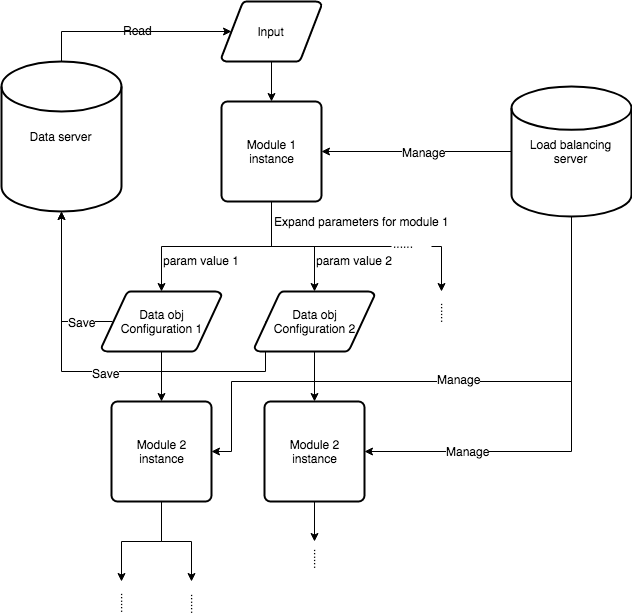
\includegraphics[width=\textwidth]{fig/control_flow.png}
        \end{center}
        \caption{Control flowchart.}\label{fig:control_flow}
    \end{figure}

    \begin{figure}[h]
        \begin{center}
            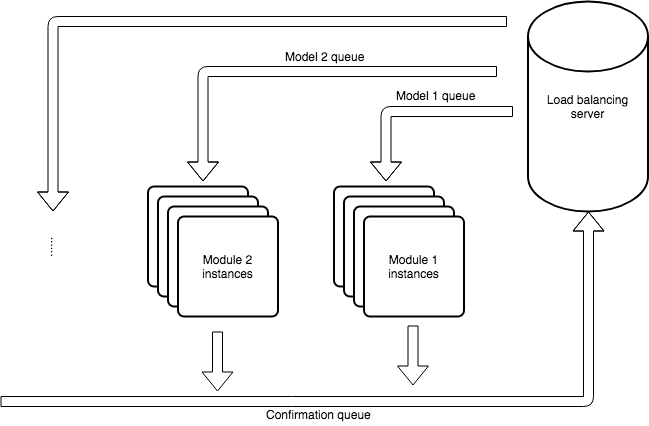
\includegraphics[width=\textwidth]{fig/information_flow.png}
        \end{center}
        \caption{Information flowchart.}\label{fig:information_flow}
    \end{figure}


    Every module runs on an independent process
    and communicates through RabbitMQ using the job class (defined in section \ref{sec:job}) which contains parameters, current excuetion status and the path to input file.
    Fig. \ref{fig:information_flow} describes the information flow.
    The Load balancing Server distributes jobs to different modules' instances.
    Once the job is finished, the instance sends a confirmation to the Load Balancing Server.


    Users only need to specify the connections between modules and the parameters associated with each module,
    the framework will automatically handle the exploration and execution of the configuration space.

    \begin{figure}[H]
        \begin{center}
            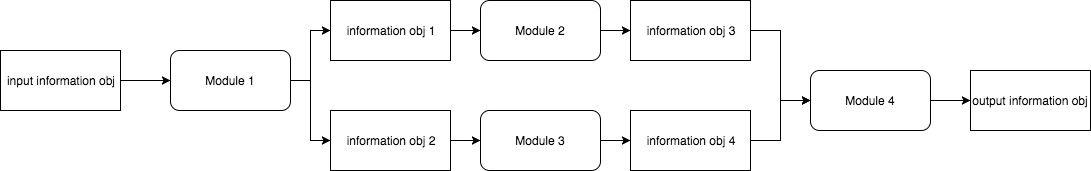
\includegraphics[width=1.2\textwidth]{fig/sample_pipeline.png}
        \end{center}
        \caption{A sample pipeline}\label{fig:sample_pipeline}
    \end{figure}
    Figure \ref{fig:sample_pipeline} shows a sample pipeline which passes the input information object
    through some modules and produces the output information object.

    We also provided a command line executable, to ease users' pain of coding.

    \subsection{Technical concerns}

        \subsubsection{Trade off between simplicity and expressiveness}
        We want to provied a simple frame work for people who need to explore some configuration spaces but don't want to spend too much time on writing complicated code.
        It is a trade off.
        If we support a lot of fancy functionalities, the code would be too hard to understand.
        We decided to implement a minimal working framework, and let users deal with the complexity caused by their own code.

        \subsubsection{Programming language}
        Since we want a simple framework, Python is the best choice.
        Because Python 3 has far better performance, we finally decided to use Python 3.

        \subsubsection{Message queue}
        The reason we used RabbitMQ is that it provides a simple, lightweight and reliable solution to pass messages through processes or different machines.

        \subsubsection{Parameter types}
        We support 3 types of parameters: int, float and collection.

        \subsubsection{Data storage}
        We support 2 types of data: a plain file on disk or a file from MongoDB.
        MongoDB's virtual filesystem, GridFS, can be accessed as long as there's internet connection.
        This functionality is crucial to migrating the application to clouds like AWS.

    \subsection{Pipeline}
    The pipeline class manages modules and parameters.
    It reads the configuration file, creates the pipeline and is the class that implements the Load Balancing Server.
    The pipeline can't have branches or merges, and the order of the configuration file should be the same as the actual pipeline.

    \begin{figure}[h]
        \begin{center}
            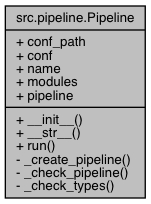
\includegraphics[width=0.3\textwidth]{fig/pipeline_uml.png}
        \end{center}
        \caption{UML diagram for the pipeline class.}\label{fig:pipeline_uml}
    \end{figure}

    \subsection{Module}
    A module is the basic computation unit which takes an input and produces an output.
    Every input and output is a job object defined in sec. \ref{sec:job}.

    A module needs to maintain the following fields:
    \begin{itemize}
        \item Name of the module.
        \item Number of instances.
        \item Configuration of the pipeline.
    \end{itemize}

    When running, the pipeline will send jobs to module instances.

    \begin{figure}[H]
        \begin{center}
            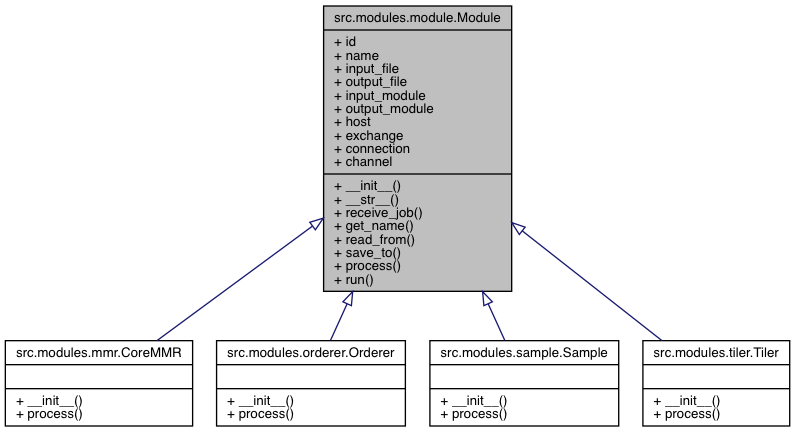
\includegraphics[width=0.4\textwidth]{fig/module_uml.png}
        \end{center}
        \label{fig:module_uml}
        \caption{UML diagrams for the abstract module class and derived classes.}
    \end{figure}

    \subsection{Parameter}
    \label{sec:parameter}
    The parameter class manages one parameter.
    It should handle all operations related the parameter,
    including updating the parameter value,
    set and reset the value.
    There are several types of params: integer, float and collection.

    It also needs to save maintain the following fields:
    \begin{itemize}
        \item Name of the parameter.
        \item Type of the parameter: int, float or collection.
        \item Interval of possible values or possible values of a collection.
        \item Step size of the parameter (for numerical params).
    \end{itemize}

    \begin{figure}[H]
        \begin{center}
            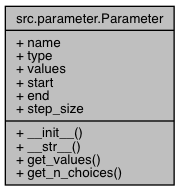
\includegraphics[width=0.3\textwidth]{fig/param_uml.png}
        \end{center}
        \label{fig:param_uml}
        \caption{UML diagram for parameter class.}
    \end{figure}

    \subsection{Job}
    \label{sec:job}
    The job class is the information object used between modules.
    It maintains the following fields:

    \begin{itemize}
        \item Job id: the unique id of the job.
        \item Producer: the module that produced this information object.
        \item Consumer: the module that this information object to be passed to.
        \item Input uri: the uri to the data file.
        \item Output path: the path to store the resulting data file.
        \item Params: the params that the module should use to process the data object.
        \item Timestamp: the timestamp when the data object was created.
        \item Processing time: the time taken to process the data object.
    \end{itemize}


    \begin{figure}[H]
        \begin{center}
            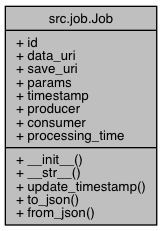
\includegraphics[width=0.3\textwidth]{fig/job_uml.png}
        \end{center}
        \label{fig:job_uml}
        \caption{UML diagram for job class.}
    \end{figure}


    \subsection{Configuration file}
    We use YAML files to configure the framework.

    \subsection{User defined modules}
    Users need to put their module classes in a file in the same folder with the configuration file.
    Then the framework will automatically load them.

    \subsection{Executable}
    We provide an executable that reads in the configuration file, and starts the whole pipeline.
    It reads the configuration file and extracts needed infomation.
    Then according to the configuration, it generates code for each module and execute the code using different processes.


\section{Example pipeline}
    This pipeline consists of a sample module,
    which does nothing but adds its own configuration and parameters to the data to show this pipeline is working.

    \begin{figure}[H]
        \begin{center}
            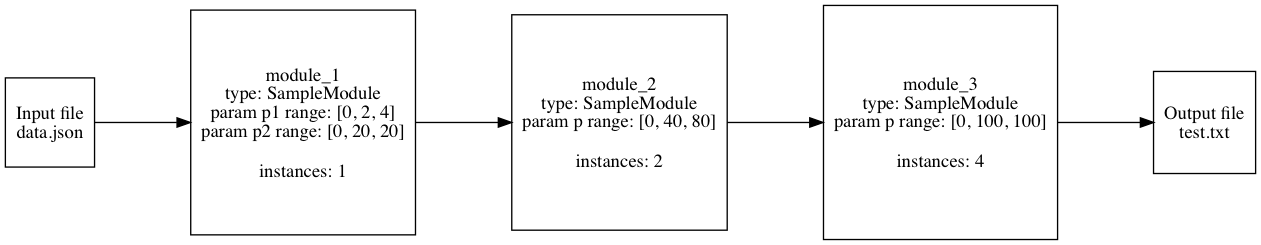
\includegraphics[width=1.2\textwidth]{fig/toy_pipeline.png}
        \end{center}
        \label{fig:toy_pipeline}
        \caption{The structure for toy pipeline}
    \end{figure}



\section{BioASQ Experiment}

    \subsection{The BioASQ Competition}
    The BioASQ Competition is a Question Answering challenge in which competitors are tasked with developing a system capable of answering a biomedical question when provided
    excerpts from relevant research papers. .

    \subsection{The OAQA BioASQ Pipeline}
    The OAQA BioASQ Pipeline \cite{chandu2017tackling} is a highly modularized pipeline developed at Carnegie Mellon University as part of the BioASQ Competition. It performs
    extractive summarization to generate responses to questions in the biomedical domain. It is composed of modules that perform candidate selection, candidate ranking, sentence ordering,
    and sentence tiling. We used the OAQA BioASQ pipeline as a use case to guide development of BOOM and performed all our intitial experiments and benchmarking on the OAQA BioASQ pipeline.

    \subsection{Implemented Modules}
        Table \ref{tbl:modules} listed all modules and their parameters we implemented.
        We have also made modifications to the BioASQ pipeline in the process of adapting it to work with our framework.
        First, because the modules each need to run hundreds of times, we have made performance improvements where we could. This includes
        making a multi-process CoreMMR module, (the most computation heavy module) that is more than 4x faster than the original module (depending the configuration).
        We have also had to refactor the way the data gets passed along the pipeline because each module needs to handle all data in order to pass it
        along to the next module, rather than only being passed the data relevant to its own functionality.

        \begin{table}[h]
            \centering
            \begin{tabular}{|l|l|}
                \hline
                Module  & Parameters \\ \hline
                CoreMMR & $\alpha$           \\ \hline
                Orderer &  k          \\ \hline
                Tiler   &  word\_limit          \\ \hline
                Rouge   &            \\ \hline
            \end{tabular}
            \caption{Table of implemented modules.}
            \label{tbl:modules}
        \end{table}

    \subsection{Pipeline}
        \begin{figure}[H]
            \begin{center}
                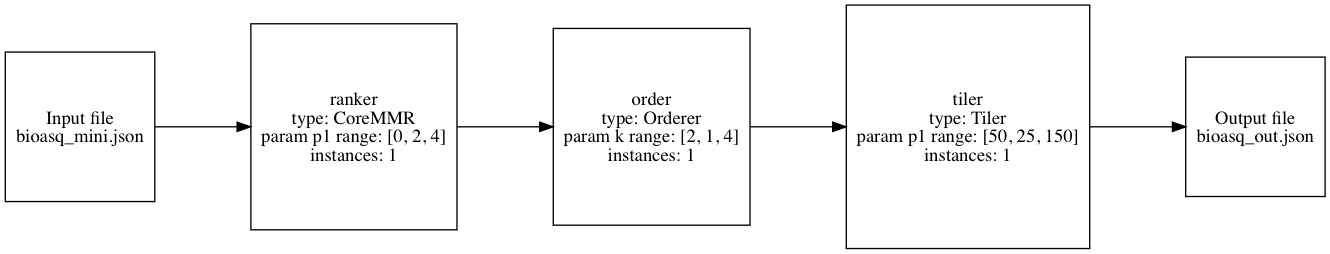
\includegraphics[width=\textwidth]{fig/bioasq_pipeline.png}
            \end{center}
            \label{fig:bioasq_pipeline}
            \caption{The structure for BioAsq pipeline}
        \end{figure}

    \subsection{Dataset}
    The results were run on a subset (1800 total questions) of the bioasq\_train\_formatted.json dataset.


    \subsection{Results}

    Our configuration tested 2688 unique parameter combinations.
    Fig. \ref{fig:histogram} shows the distribution of the 2688 Rouge scores that resulted from the configuration space exploration.
    The results clearly show that for BioASQ have two distinct clusters of scores, one for which the Rouge score is between 0.24 and 0.26,
    and the second with scores between 0.28 and 0.32.

    \begin{figure}[H]
        \begin{center}
            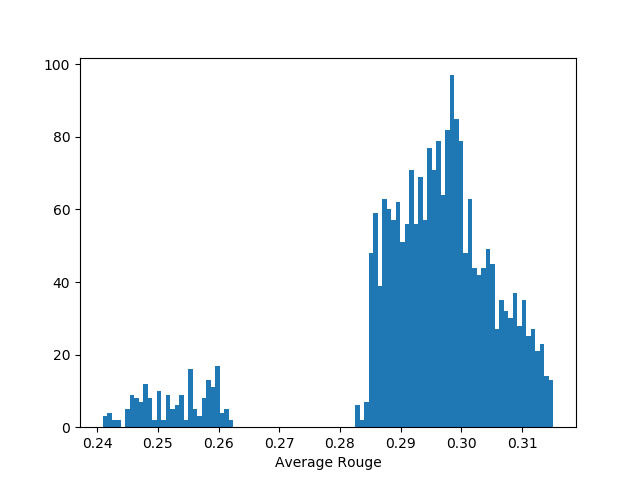
\includegraphics[width=\textwidth]{fig/hist.png}
        \end{center}
        \caption{The distribution of scores across all 2688 parameter configurations}\label{fig:histogram}
    \end{figure}

    \begin{figure}
        \begin{tabular}{lc}
             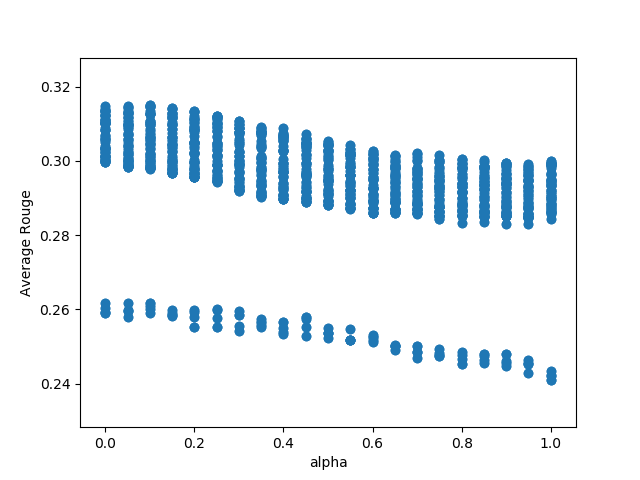
\includegraphics[width=50mm]{fig/alpha.png} &   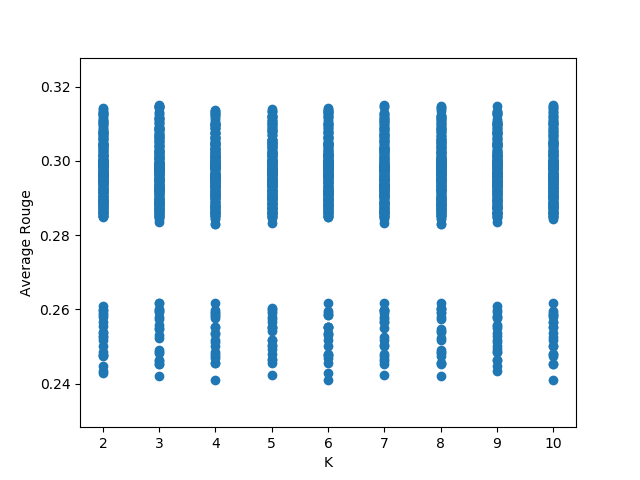
\includegraphics[width=50mm]{fig/k.png} \\
            (a) Average Rouge score vs. alpha  & (b) Average Rouge score vs. k (number of clusters) \\[10pt]
            \multicolumn{2}{c}{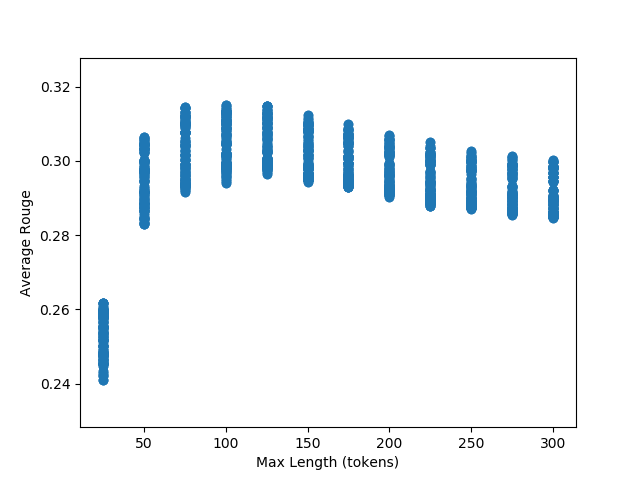
\includegraphics[width=50mm]{fig/wordcount.png} }\\
            \multicolumn{2}{c}{(c) Average Rouge score vs. word limit}
        \end{tabular}
        \caption{Distribution of Rouge scores against each individual parameter}\label{fig:ind_plots}
    \end{figure}

    Looking at each parameter plotted individually, as in Fig. \ref{fig:ind_plots}, we can see that the separate clusters of scores are entirely explained by the word limit parameter.

    The results showed that he alpha parameter (Fig. \ref{fig:ind_plots}a) showed noticeable penalties for values greater than 0.2, although as a penalty for repetition higher values may score better on a human-evaluated readability metric.

    The K parameter (Fig. \ref{fig:ind_plots}b) used in the KMeans clustering to perform sentence ordering does not have a large impact on the results.
    This is intuitive since the purely reordering the sentences does not affect the Rouge score unless a sentence is moved to the end and clipped due to the maximum length requirement.

    The maximum length parameter (Fig. \ref{fig:ind_plots}c) has by far the biggest impact on the results with a huge penalty for allowing fewer than 75 tokens, but also a decrease at greater than 150.

    \begin{figure}[H]
        \begin{center}
            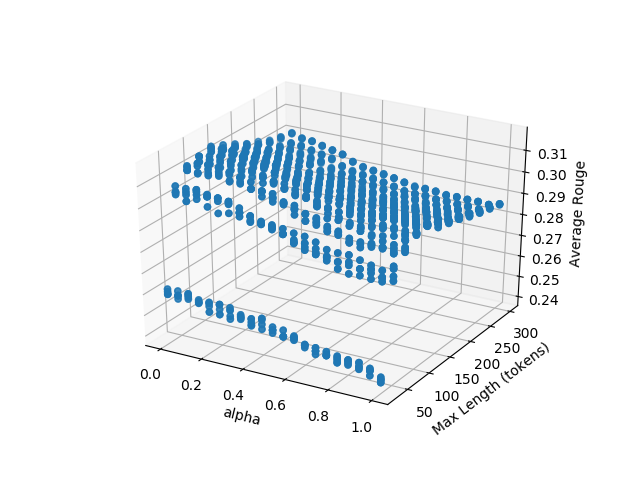
\includegraphics[width=\textwidth]{fig/alpha_wordcount.png}
        \end{center}
        \caption{The distribution of against both word\_limit and alpha}\label{fig:alpha_wordcount}
    \end{figure}

    Fig. \ref{fig:alpha_wordcount} shows Rouge score plotted against both the alpha parameter and the word\_limit parameter, the two parameters with the most influence over the Rouge score.
    This graph shows the interaction of the two parameters and and encompasses the vast majority of the variation in Rouge score since the k parameter has a negligible impact. From this graph,
    we can see that the maximum Rouge score appears where the alpha is low (<0.2) and the word\_limit parameter is in the range of 100-150 tokens.

    Our experimental results show that the best configuration for the existing BioASQ pipeline uses the following parameters: alpha=0.10, k=3, word\_limit=100.


\section{Future Work}
    \subsection{Job-level profiling}
    We need to profile each job to know the performance bottleneck of a pipeline.
    So that we could configure the pipeline differently to optimize its performance.

    \subsection{Automatical load balancing}
    We hope to control all modules automatically according to the performance of each module.

    \subsection{Better method to start/stop modules}
    To manage a cluster, we need different method to start/stop modules on different machines and also different methods to distribute code to each machine.

    \subsection{Fully support for using cloud}
    We have supported MongoDB to store data, but we need more components to fully support running on the cloud.

    \subsection{Intelligently search the space}
    Instead of requiring the user to define not only the parameter space, but also the regular interval at which the space is sampled, the framework should be able
    to randomly sample the space at a low resolution and then make its own decision about which regions of the space to sample more finely based on the initial results.

    \subsection{Modules as parameters}
    The framework should provide a way to swap out modules as part of the configuration space. Currently, module behavior can be controlled using a collection type parameter
    and behavior can be altered based on the parameter passed to the module. In this way we can simulate the effect of swapping out different modules, but if the modules
    have different parameters associated with them then redundant parameter configurations will be generated since the framework generates all possible parameter configurations.
    The framework should offer more support for these kinds of configurations where parameters should be generated as pairs and certain configurations are not relevant.

\section*{Acknowledgements}
Thank you to Khyathi Chandu for her assistance.


\bibliographystyle{abbrv}
\bibliography{ref}


\end{document}
